\begin{figure}
	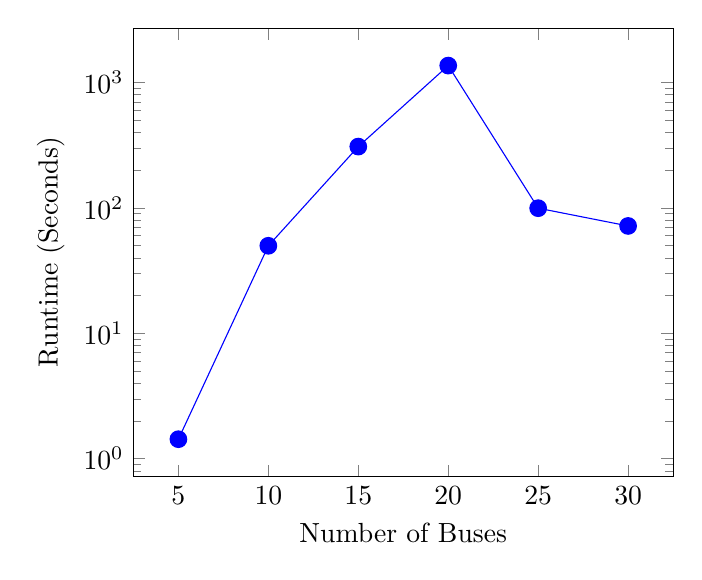
\begin{tikzpicture}
		\begin{axis}[xlabel=Number of Buses, ymode=log, ylabel=Runtime (Seconds)]
			\addplot[blue] coordinates {
				(5,  1.43  )
				(10, 49.92 )
				(15, 308.80)
				(20, 1367.0)
				(25, 99.59 )
				(30, 71.86 )};
			\addplot[blue, only marks, mark size=3pt] coordinates {
				(5,  1.43  )
				(10, 49.92 )
				(15, 308.80)
				(20, 1367.0)
				(25, 99.59 )
				(30, 71.86 )}; 
		\end{axis}
	\end{tikzpicture}
	\caption{Runtime with 5 Chargers at a 7\% Gap}
	\label{fig:scalabilityRuntime}
\end{figure}


